\documentclass[12pt, a4paper]{article}
\usepackage{titlesec}
\usepackage{graphicx}
\usepackage{amsmath}
\usepackage{geometry}
\usepackage[unicode]{hyperref}
\geometry{
    a4paper,
    lmargin=30mm,
    rmargin=20mm,
    tmargin=20mm,
    bmargin=20mm
}
\renewcommand{\figurename}{Att.}
\titlelabel{\thetitle.\quad}
\author{Pēteris Račinskis pr20015}
\date{05/01/22}
\begin{document}
\title{Praktiskais darbs - Eirovīzija}

\clearpage
\maketitle
\thispagestyle{empty}
\clearpage
\setcounter{page}{1}
\newpage

\textit{Piebilde:} praktiskā darba nosacīijumos nav norādīts sagaidāmais atskaites apjoms. Kursa aprakstā tas tiek saukts par kursa darbu, kas liecina, ka tiek gaidīts aptuveni 15-30lpp. garš dokuments ar atbilstošu ieguldītā darba un informācijas apjomu. Atvainojos, ja iesūtītā atskaite ir ievērojami plānāka, nekā tiek gaidīts - taču kaut kāds darbs ir padarīts, vairākas dienas laika ir iztērētas, personīgais sesijas grafiks liek virzīties tālāk pie citiem uzdevumiem, un, ja pastāv kaut neliela iespēja uzlabot gala vērtējumu, uzskatu, ka ir vērts iesūtīt pat potenciāli nepietiekamu rezultātu.

Visi koda faili, attēli, datu korpusi: \href{https://github.com/peteris-racinskis/DIA_PD}{GitHub - DIA\_PD}

\section{Ievads}

\subsection{Uzdevums}
Datizraces uzdevumi var būt dažādi. Viens no veidiem, kā tie var radikāli atšķirties pēc būtības, ir pirms pētījuma sākšanas pastāvošā skaidrība par rezultāta formu. Ja kādreiz sākam ar datu kopu, par ko nekas nav zināms, un mēģinām gūt vispārīgus priekštatus par starp tās elementiem pastāvošajām sakarībām, citreiz jau no paša sākuma ir laba izpratne par to, ko vēlamies sasniegt, kādi ir datu kopu veidojošie mehānismi un kādus skaitļus varētu redzēt iegūto aprakstošo modeļu parametros. Šis uzdevums visai pārliecinoši pieder otrajai kategorijai. Prasīts atbildēt uz ļoti specifisku jautājumu. Tāpēc tā vietā, lai sāktu ar ļoti vispārīgu datizraces metožu lietojumu, varam pielāgot vai izstrādāt darba rīkus tieši viena jautājuma atbildēšanai. Turklāt jautājums uzdots par datu kopas ģenerējošo procesu - eirovīzijas dziesmu konkursu - nevis par kādu konkrētu, specifiskā veidā strukturētu korpusu, kas ļauj patstāvīgi izvēlēties maksimāli piemērotu informācijas avotu, ierobežot definīcijas apgabalu pēc saviem ieskatiem, u.t.t.

Intuitīvi uzreiz rodas priekštats, kas domāts ar terminiem "kaimiņu būšana" un "objektīvāks novērtējums". Taču ar to nepietiek, lai iegūtu kaut kādu šo fenomenu skaitlisku izteiksmi. Nepieciešams definēt "objektīvu novērtējumu" un attiecīgi - novirzes no tāda. Viens veids, kā to darīt, varētu būt ieviest latentu dziesmu "popularitātes" mēru. Tādu var modelēt, iztēlojoties "demokrātisku" visu skatītāju balsošanu par, viņuprāt, labāko konkursa kārtas dalībnieku dziesmu:

\begin{equation}
 i \in \lbrace 1,2,...,K \rbrace = [K]
\end{equation}

\begin{equation}
    N_i - \text{balsis par dziesmu}; N - \text{balsis kopā}
\end{equation}

\begin{equation}
    q_i = \frac{N_i}{N}; \sum_{i\in[K]} q_i = 1
\end{equation}

\begin{equation}
    s_i \in [10] \cup 0 - \text{punktu skaits (score)}; s_i \sim P(s_i = x \mid q_i, K)
\end{equation}

\begin{equation}
    q_i \leq q_j \Rightarrow s_i \leq s_j
\end{equation}
\begin{equation}
    s_i, s_j \neq 0 \Rightarrow s_i \neq s_j
\end{equation}


kur $P(x \mid q_i, K)$ ir sadalījums, kas apraksta katra iespējamā diskrētā novērtējuma (punktu skaita) varbūtību, pieņemot, ka dziesmas "demokrātiskā" balsojuma varbūtība ir $q_i$. Šķiet, ka šis sadalījums varētu kaut kādas formas binomiālais, (vai arī kaut kas krietni sarežģītāks), taču tā precīzā analītiskā forma nav svarīga tālākiem aprēķiniem. Svarīgi piebilst, ka eirovīzijas vērtējumu sistēmā parasti punkti pieder kopai $[8] \cup \lbrace 0, 10, 12 \rbrace$, un šīm skaitliskām vērtībām ir nozīme, rēķinot gala rezultātu (punkti tiek skaitīti kopā), taču katras dalībvalsts vērtējuma piešķiršanas procesā šiem skaitļiem ir tikai ordināla nozīme, t.i., $10<12$; $\forall i \in [8]: i < 10$. Tāpēc var pieņemt, ka $s_i \in [10]$ un vajadzības gadījumā izmantot pārveidojumu $\hat s_i = f(s_i); f(9)=10;f(10)=12;f(x \neq 9,10)=x$.

Tad sagaidāmo punktu skaitu, ja balsojums notiek tikai vienreiz un sakrīt ar "objektīvo" novērtējumu (vienā valstī, visās kopā), var izteikt kā:

\begin{equation}
    E[s_i^1] = \sum_{s\in[10]}P(s\mid q_i, K)*s
\end{equation}

bet, ja balsojums tiek atkārots vairākas reizes un tiek skaitīta to svērto variantu summa ($K'$ ir balsojošo dalībvalstu skaits, kas daudzreiz ir tāds pats, kā uzstājošos dalībvalstu skaits, bet ne vienmēr, jo nesenākos konkursos ieviesta pusfinālu sistēma un visas valstis var balsot finālā):

\begin{equation}
    E[\hat s_i^{K'}] = \sum_{j\in [K']}\sum_{s\in[10]}P(s\mid q_i, K)*f(s)
\end{equation}

Ja interesē nevis dziesmas rezultāts konkursa uzvarētāja noteikšanai, bet tās vidējā ordinālā pozīcija katras balsotājvalsts vērtējumā, pārveidojumu $f(x)$ var (varētu pat teikt, ka nepieciešams) atmest. Pilnīgi korekts novērtējums šis nav tāpat, jo pazudušas ir visas vērtības, kas nav starp 10 lielākajām:

\begin{equation}
    E[s_i^{K'}] = \sum_{j\in [K']}\sum_{s\in[10]}P(s\mid q_i, K)*s = K'*E[s_i^1]
\end{equation}

Kā redzams, rezultāts nav atkarīgs no katras dalībvalsts un ir "objektīvs". Ieviest nobīdes nacionālajos balsojumos varētu ar svariem:

\begin{equation}
    E[s_i^{K'}] = \sum_{j\in [K']}E[s_i^{1}]*w_{ji}, \sum_{i\in[K]} w_{ji} = 1
\end{equation}

un tad "neobjektivitāti" varētu potenciāli labot, lai atjaunotu sagaidāmo vērtību, reizinot svarus ar korekcijas koeficientiem, kas iegūti, dalot svarus ar vienmērīgam sadalī-jumam (pār vērtējamām dalībvalstīm, nevis balsojošajām) atbilstošajiem:

\begin{equation}
    c_{ji}=\frac{w_{K}^0}{w_{ji}}=\frac{\frac{1}{K}}{w_{ji}}=\frac{1}{K*w_{ji}}
\end{equation}

un visu kopā apkopot korekciju matricā:

\begin{equation}
    C=
    \begin{bmatrix}
        c_{11} &  ... & c_{1K'} \\
        \vdots & \ddots & \vdots \\
        c_{K1} &  ... & c_{KK'} 
    \end{bmatrix}
\end{equation}

Lai šo korekciju matricu pielietotu rezultātu labošanai, punktu matricu (bez $f(s)$ pārveidojuma) pa elementiem reizina ar korekciju matricu:
\begin{equation}
    S=
    \begin{bmatrix}
        s_{11} &  ... & s_{1K'} \\
        \vdots & \ddots & \vdots \\
        _{K1} &  ... & s_{KK'} 
    \end{bmatrix}
\end{equation}
\begin{equation}
    S' = C \circ S
\end{equation}

Kas tad īsti ir iegūts, un kā no tā aprēķināt konkursa rezultātu? Jāatceras, ka $s_i$ ir punktu skaits, kas iegūts, pēc slēptā mainīgā $q_i$ kārtojot konkursa dalībniekus un piešķirot punktus 10 labākajiem. Ir izdarīts pieņēmums, ka katra valsts vispirms ieguvusi šos punktu skaitus no vienādiem varbūtību sadalījumiem, tad pareizinājusi ar svariem. Koriģējot, atgriezta pēdējā darbība, un iegūti punktu skaiti, kādi tie būtu pirms šīs fiktīvās svēršanas operācijas, pēc fiktīvas demokrātiskas balsošans un punktu piešķiršanas. 

Protams, ka realitātē process ir citāds: svari netiek pielietoti punktiem, tā vietā jau punktu skaitu sadalījums ir kropļots - precīzākus rezultātus varētu iegūt, rēķinot korekcijas saņemto balsu skaitiem, ja tie būtu zināmi (un nebūtu žūrijas komponentes, kas visu šo "demokrātijas" modeli padara par vienkārši nederīgu). Turklāt visas vērtības, kas nav bijušas augstākajā desmitniekā no datu kopas vienkārši ir izgrieztas (vienādas ar 0). Tāpēc jau uzreiz var pateikt, ka no matemātiska viedokļa, ar šādu matricu nav iespējams atjaunot slēpto $q_i$ sadalījumu. Taču no statistikas kursa pagājušajā semestrī zināms, ka t.s. "rangu" metodes, kas strādā ar kārtas skaitļiem, nevis skaitliskām vērtībām tiešā veidā, parasti uzvedas vismaz virpsusēji līdzīgi nepārtrauktajām, un bieži vien ir algoritmiski vienkāršākas (pat ja kaut ko par tām pierādīt mēdz būt grūtāk), tāpēc var pastāvēt zināma cerība, ka pat matemātiski nekorektas un nepilnīgas, no datu korpusiem ar iztrūkumiem iegūtas korekcijas varētu darboties vismaz pareizajā virzienā.

Attiecīgi tiek izvirzīts sekojošs korekcijas modelis: tā kā iegūtas ir "atjaunotās" rangu sagaidāmās vērtības, tās drīkst vienkārši pārkārtot - piešķirt kārtas skaitļus no mazākās uz lielāko - un izdarīt korekciju $f(s)$, lai svērtu kārtas skaitļus summās starp balsojošajām valstīm.
\begin{equation}
    S'' = S' \text{ rangos 1-10 (pārējie = 0), pa kolonnām}
\end{equation}
\begin{equation}
    \hat S'' = f(S'')
\end{equation}
\begin{equation}
    \hat s_i = \sum_{j \in [K']}\hat s_{ij}
\end{equation}


Jāmin, ka šādi nav iespējams izšķirt tieši "kaimiņu būšanu" - ko varbūt gribētos rakstu-rot kā tīri etniskas tuvības vai ģeopolitisku interešu sakritības motivētu nobīdi balosjumu rezultātos. No citiem faktoriem, kas arī atšķiras valstu starpā - kulturālas noslieces, demogrāfiskie sadalījumi, konkursa popularitāte, u.t.t. - radušās nobīdes skaitliski izskatītos tāpat. 

\subsection{Datu kopas}

Kā jau minēts iepriekš, uzdevums ir par fenomenu, nevis tā radītu konkrētu datu kopu. Tāpēc iespējams ne tikai brīvi pēc saviem ieskatiem pārveidot vienu datu kopu, bet apzināti meklēt un izvēlēties jau maksimāli atbilstoši noformētu. Nav arī dots stingrs uzstādījums, ka obligāti jāstrādā ar visu konkursa vēsturi. Laika gaitā ir notikušas daudzas noteikumu un organizatoriskas izmaiņas, kas var apgrūtināt dažādu periodu rezultātu salīdzināšanu.

Par datu kopu izvēlēta \textit{Eurovision Song Contest Dataset} \href{https://github.com/Spijkervet/eurovision-dataset}{(pieejama \textit{GitHub} repozitorijā)}, kur jau atrodams korpuss \textit{votes.csv}. Tajā katrā rindā dots notikuma gads, atbilstošā stadija (fināls; pusfināls; pirmais vai otrais pusfināls gados, kad ir divi), vērtējošā valsts un punktus saņemošā valsts. 

Pietiek vien atvērt \href{https://en.wikipedia.org/wiki/Voting_at_the_Eurovision_Song_Contest}{\textit{Wikipedia} rakstu par konkursa balsošanas kārtību}, lai kristu nelielā panikā. Garākais (un, Latvijas iedzīvotājiem, interesantākais) posms ar samērā noturīgu balsošanas kārtību ir 1980-2015, tāpēc tālāk tieši ar to arī pārsvarā strādāts.

\newpage
\section{Metodes}

\subsection{Modeļi}

Sadaļā 1.1. aprakstīts, kā varētu izskatīties korekcijas matrica, un radīta aptuvena nojausma par procesu, kas šādu matricu varētu ģenerēt, taču tā nav konstruktīva - svari $w_{ji}$ \textit{a priori} nav zināmi, tos nepieciešams noteikt empīriski. Līdz šim arī aplūkots tikai gadījums ar vienu $q_i$ "kvalitātes vērtību" sadalījumu. Dažādās konkursa kārtās šie sadalījumi var radikāli atšķirties. Vienam konkursa etapam korekcijas varētu vienkārši algebriski izrēķināt, taču, ja vēlamies noteikt korekcijas matricu $C$ noteikt globāli, jāveido modeļa šablons un jāapmāca.

Var krietni palauzīt galvu, domājot par veidiem, kā to izdarīt. Pirmā ideja, kas varētu rasties, varētu būt vienkārši ņemt punktus tiešā veidā no datu kopas un apmācīt klasifikatoru formā (vērtējošā valsts, vērtējamā valsts) $\rightarrow$ vērtējums (kur vērtējums vai teksta mainīgai, vai diskrētu vērtību vektors, kur 1 apzīmē konkrētu punktu skaitu). Lai iegūtu sagaidāmās vērtības novērtējumu, var izmantot daudzu klasifikatoru īpatnību - modeļa ģenerētais izejas vektors var tikt normalizēts uz varbūtību sadalījumu, nevis vienu konkrētu klasi. Šīs varbūtības tad var reizināt ar atbilstošajām punktu vērtībām, lai iegūtu matemātisko cerību. Problēma ar šādu pieeju ir tāda, ka bieži vien pieejami pavisam nedaudzi novērtējumi no vienas valsts uz otru. Par spīti šim trūkumiem, mēģinājumi uztrenēt klasifikatora šablonu datu kopai tika veikti, bet vienīgais, kas sniedza cilvēkam saprotamus rezultātus, bija neironu tīkls. Iegūtās sagaidāmās vērtības var tikt izmantotas kā distances starp dalībvalstīm vai par estimatoru, no kā tālāk rēķināt korekcijas. Citi izmēģinātie modeļu šabloni bija SVM un \textit{NaiveBayes}, taču ar tiem semantiski saprotamas skaitliskas vērtības gūt neizdevās, un tiem atbilstošais kods ir izkomentēts.

Tā kā neviens no tipveida modeļu šabloniem nešķita ideāli piemērots tieši šim uzdevumam, pirmais algoritms, kas tika realizēts, bija paša rakstīts. Tā vietā, lai pakāpeniski optimizētu šablonu, iterējot pār datu kopas elementiem, datu kopu var mēģināt reducēt uz formu, kur rezultāts atrodams algebriski. Šajā konkrētajā gadījumā tas darīts, nosakot vidējās empīriskās vērtības piešķirto punktu skaitam katram valstu pārim katrā virzienā, pārveidojot tās par divdimensionālu varbūtību sadalījumu un pielīdzinot rezultātu vien-mērīgajam sadalījumam. 

To dara, atrodot divus korekcijas koeficientus: $r_i$, kas vienādo rindu varbūtību summas (savā ziņā kompensējot $q_i$) un $c_{ij}$, kas vienādo varbūtības koriģētās matricas kolonnās un reizē ir arī korekcijas matricas vērtības. 

\begin{equation}
    p_i=\sum_{j\in [K']}p_{ij}
\end{equation}
\begin{equation}
    p_i*r_i=\frac{1}{K}
\end{equation}
\begin{equation}
    r_i = \frac{1}{p_i*K}
\end{equation}
\begin{equation}
    p_{ij}'=p_{ij}*r_i
\end{equation}
\begin{equation}
    p_{ij}'*c_{ij}=\frac{\sum_{i\in[K]}p_{ij}'}{K}
\end{equation}
\begin{equation}
    c_{ij}=\frac{\sum_{i\in[K]}p_{ij}'}{p_{ij}'K}
\end{equation}
\begin{equation}
    w_{ij}=\frac{1}{c_{ij}K}
\end{equation}

Praktiski tika konstatēts, ka, iespējams, kvalitatīvākus rezultātus sniedz korekcijas kvadrātsakne, par ko diskutēts pie rezultātiem:
\begin{equation}
    c'_{ij} = \sqrt{c_{ij}}
\end{equation}
\begin{equation}
    S' = C' \circ S
\end{equation}


Par šī algoritma matemātisko pareizību pārliecības nav nekādas - pirmais kompensāci-jas solis koriģē $q_i$, balstoties uz stipri kropļotiem vērtējumiem, un svari tad tiek rēķināti no šī nekorektā starprezultāta. Taču vismaz virspusēji šķiet, ka iegūie rezultāti varētu būt noderīgi. 

Iespējams, ka varētu šo procesu pilnveidot, ieviešot iterāciju un cerot uz konverģenci, atkārtoti veicot korekcijas aprēķinu koriģētiem datiem, taču matemātiski pamatot, kāpēc tam būtu jāstrādā, laika nav pieticis. Galvenais šķērslis ir šaubas par to, kā pareizi kombinēt soļos iegūtās korekcijas matricas - vai tas vispār ir pamatojams. Taču zināms, ka līdzīgas metodes izmanto citur datizracē, lai cīnītos ar t.s. \textit{distribution shift} jeb atšķirību starp modeļa ģenerētiem sadalījumiem un reāliem.

\subsection{Datu priekšapstrāde}

Klasifikatoru šablonu izmantošanai nepieciešams datu kopu "vektorizēt", t.i., diskrētas klases ieejas datu kopā izteikt kā vektorus ar vienu nenulles elementu. Atkarībā no konkrētā algoritma realizācijas, var būt nepieciešams rezultātu kolonnu vai nu izteikt kā tādu pašu vektoru, vai viendimensionālu sarakstu ar teksta elementiem. Šīs manipulācijas veic \textit{Python} skripts \textit{vectorize.py}, pieejams kopā ar visiem pirmkoda failiem un dažādiem datu apstrādes starpproduktiem projekta repozitorijā.

Lai veiktu aprēķinus pēc algebriskās metodes, jāveic smagnējāki pārveidojumi. Kopu ar kortežiem formā $(t,i,j,s)$ nepieciešams izteikt kā tensoru ar elementiem $s_{ijt}$, kur $t$ - konkursa etaps. Ja konkursa etapu dalībnieki un balsotāji vienmēr būtu tie paši, šis būtu triviāls uzdevums. Taču sarežģījumus rada fakts, ka neeksistējošas vērtības un nulles vērtības nav viens un tas pats. Ne katra dalībvalsts piedalās katrā etapā un ne katra dalībvalsts, kas balso, arī piedalās konkursā. Tāpēc neeksistējošas vērtības nepieciešams marķēt atsevišķi. Izvēlētais risinājums ir tās marķēt ar $-1$, un pēc tam datu apstrādē īpaši apstrādāt šādi marķētus ierakstus, kur nepieciešams. Vērtībām 10,12 tiek ieviesta jau iepriekš aprakstītā korekcija uz 9,10.

Šīs operācijas veiktas repozitorijā pieejamajā skriptā \textit{datagen.py}. Principā
priekš-apstrādes solī iespējams arī veikt vidējo vērtību rēķināšanu, kas droši vien arī būtu ātrāk nekā faktiski realizētajā tensora ģenerēšanas pieejā, taču tīri praktiski apsvērumu vadībā tika izlemts visas netriviālās datu manipulācijas atstāt atsevišķi: darba autors daudz labāk pazīstams ar n-dimensionālu homogēnu datu bloku skaitļošanas un lineārās algebras bibliotēku \textit{numpy} nekā ar 2-dimensionālu heterogēnu datu korpusu apstrādes bibliotēku \textit{pandas}. Izstrādes procesā vieglāk iteratīvi izmainīt visu procesu, strādājot ar jau gatavu datu tensoru. Lai nebūtu katru reizi jāveic tensora veidošana, kas aizņem gandrīz 40 sekundes, starprezultāts tiek saglabāts failā. Datu pārveidošanu ir iespējams paātrināt daudzkārtīgi, taču tad jāizmanto cita darbību secība, ko grūtāk atkļūdot. Reizi dažās stundās zaudēt 40s šķiet mazāks zaudējums, nekā pavadīt vairākas stundas, pārrakstot jau pietiekami labi strādājošu kodu. 

Šī ir arī laba vieta tekstā, kur norādīt, ka šādam datu formātam matrica ar vērtējoša-jām un vērtejamām valstīm vienmēr ir kvadrātiska, t.i., $K = K'$. Iztrūkstošās šķautnes ir atbilstoši marķētas ar vērtībām ārpus parastā definīcijas apgabala..

\subsection{Modeļu aprēķins}

Universālo klasifikatoru apmācībai izmantota bibliotēka \textit{scikit-learn}, kas ļauj ar ļoti lako-niskām definīcijām pielietot dažādus visai jaudīgus datizraces algoritmus. Ja nav vēlmes vai nepieciešamības īpaši iedziļināties modeļu hiperparametru optimizācijā, šādu rīku izmantot ir vienkāršāk nekā daudz jaudīgākas bibliotēkas kā \textit{tensorflow}. Kods atrodams skriptā \textit{model-classifier.py}. Tā kā šī programma rakstīta vēlāk, tā vietām izmanto funkcijas no zemāk aprakstītās.


Algebriskā modeļa aprēķins tiek veikts citā \textit{Python} skriptā - \textit{model.py}. Pirms iespējams aprēķināt vidējās vērtības pār etapiem, nepieciešams noteikt katra balsojuma virziena (varētu teikt, orientēta grafa šķautnes) kopskaitu. To veic funkcija \textit{coincidence\_count}, kas atgriež matricu ar vērtībām formā $n_{ij}$ - reižu skaits, kad j-tā valsts balsojusi konkursā, kurā uzstājas i-tā. Šo parametru izmanto funkcija \textit{clear\_dataset}, kas atsijā valstis pēc sliekšņa kritērija - ja maksimālais $n_{ij}$ ir mazāks par slieksni, no matricas tiek izmestas i-tās rindas un i-tās kolonnas. Tādējādi tiek apkarota traucējoša parādība - valstīm, kas piedalījušās konkursā tikai dažas reizes, korekcijas koeficienti var būt krietni lielāki vai mazāki, nekā visām pārējām, jo lielo skaitļu likumam nav pieticis elementu, lai izlīdzinātu iegūto punktu skaitus un tuvotos sagaidāmajai vērtībai. Piešķirto punktu summu atrod funkcija \textit{coincidence\_total}. Vidēji j-tās valsts i-tajai piešķirto novērtējumu tad atrod \textit{edge\_average}. 

Nākamais solis ir iegūto vidējo vērtību pārveidošana par varbūtību sadalījumu. Sāku-mā tas netika darīts, un rezultāts bija grūtības ar izsekošanu vērtību semantiskajai nozīmei un pareizu algoritma realizāciju. Strādājot ar varbūtībām, daudzas potenciālas programmatiskas kļūdas var novērst, vienkārši sekojot līdzi tam, ka rindu, kolonnu vai kopējā varbūtību summa matricā ir vienāda ar 1 (atkarībā no veicamajām darbībām). Papildus tiek veikts arī matemātiski pilnīgi nepamatots taču praktiski pašsaprotams solis - visām vidējo vērtējumu matricas vērtībām tiek pieskaitīta konstante $\alpha$, kas ir funkcijas parametrs. Tas tiek darīts, jo citādi nogrieztām vērtībām tiek aprēķināts svars 0 un korekcijas koeficients $+\infty$, kas korekcijas mērķiem neder. To var uztvert kā zaudētās informācijas ekstrapolāciju - valstis, kas ne reizi nav saņēmušas rangu 1-10, tik un tā gandrīz noteikti kādas balsis saņemtu, ja tiktu veikta izlase no balsis veidojošā sadalījuma. Visu augstāk minēto veic funkcija \textit{normalized\_score}.

Tālāk, 2.1. sadaļā aprakstīto korekcijas matricas aprēķinu veic funkcija \textit{corrections}. Strādājot ar \textit{numpy}, mēdz rasties nepieciešamība veikt skalāras operācijas starp vektoriem, matricām un dažādu dimensiju tensoriem - un tad var pieļaut grūti atrodamas kļūdas, nepareizā secībā savietojot to dažādās dimensijas. Tāpēc funkcija \textit{expand} gluži vienkārši vienreiz atrisina šo problēmu, lai vēlāk programmētājam par to nebūtu jādomā. \textit{weights} un \textit{distance\_measure} atgriež attiecīgi noteikto svaru un simetrisko distanču matricas informatīviem mērķiem. Šīs pašas funkcijas izmanto, lai apstrādātu neironu tīkla ģenerētās matemātiskās cerības.

Lai korekciju piemērotu datu kopai, izveidotas funkcijas \textit{apply\_correction\_matrix} un \textit{rank\_corrected}. Pirmā pareizina datu kopu ar korekcijām, saglabājot iztrūkstošo datu vērtības, otrā veic diezgan piņķerīgo koriģētu vērtību pārkārtošanas procedūru, ko nevar pilnībā vektorizēt (t.i, uzreiz nodot aprēķina formulu visam tensoram).

Subjektīvam novērtējumam ar tiktāl minēto pietiek - var aprēķināt matricas koeficientus, pārveidot tos par distancēm, pārbaudīt iegūtās vērtības skaitliski vai veikt ar tām dimensiju redukciju. Taču kā spriest par korekciju "pareizību"? Cik lielā mērā tās patiešām kaut ko uzlabo? Tas, protams, ir filozofisks jautājums, un droši vien pietiekami sarežģīts arī no matemātikas viedokļa. Īpaši neiedziļinoties varētu izmantot intuīciju un pieņemt, ka, ja kaut kādā veidā kompensēsim slēptus svarus, mēģinot vienādot ar tiem iegūtos rezultātus, tad šo te iegūto rezultātu dispersijai vajadzētu mazināties. Funkcijas \textit{split\_dataset} un \textit{pre\_post\_variance} realizē "slinko krosvalidāciju". Proti, viena sadala datu kopu nejauši izvēlētās apakškopās, otra aprēķina dispersiju katram tensora "slānim" un atgriež vidējās vērtības - pirms un pēc korekcijas. Lai gūtu krosvalidācijai līdzīgu efektu, šo procedūru var atkārtot daudzas reizes. Padodot par argumentu visu treniņa kopu abās ailēs, iespējams novērtēt dispersijas izmaiņas visai kopai.

Visbeidzot, iegūtos rezultātus izvada failos - distanču, svaru, korekciju matricas; valstu indeksiem atbilstošos kodus; datu tensora formu (lai varētu pareizi to atjaunot citur). Uz konsoles tiek izvadīti "krosvalidācijas" rezultāti visiem datiem, 10 neujaušiem dalījumiem, 10 tuvākās distances, 10 tālākās un Latvijai - 5 tuvākās, 5 tālākās. Repozitorijā atrodas arī skripts \textit{mds.R}, kur bez īpašām pārmaiņām pārkopēts kods no 2.1. mājas darba, lai pārbaudītu, vai ar MDS un isoMDS var iegūt vizuāli uzskatāmus rezultātus. 

\section{Rezultāti}

Tā kā neironu tīkls apmācīts uz atšķirīgas formas datu kopas, ar to nav mēģināts rēķināt "krosvalidāciju". Bet analoģiski salīdiznāt iespējams abu modeļu radītos distances mērus.

\begin{figure}[h!]
    \centering
    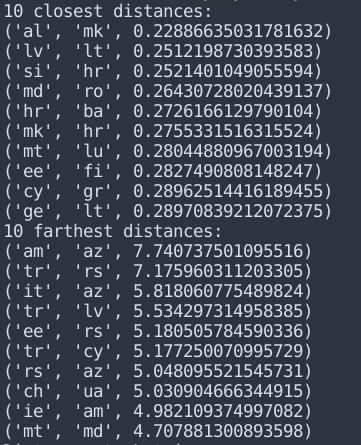
\includegraphics[height=7cm,page=1]{close-far-classifier.png}
    \caption{Klasifikatora distances}
\end{figure}
\begin{figure}[h!]
    \centering
    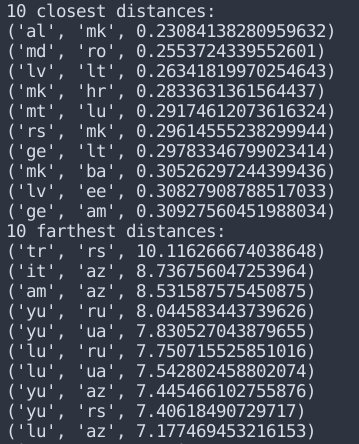
\includegraphics[height=7cm,page=1]{close-far-model.png}
    \caption{Vidējo vērtību matricas distances}
\end{figure}

Redzams, ka tuvības starp Balkānu un Baltijas valstīm abi modeļi atrod ļoti līdzīgas (skaitlisko vērtību sakritība gan ir nejauša, nozīme ir secībai - mainot parametru $\alpha$ var iegūt dažādas absolūtās vērtības), taču atšķiras valstis, ko modeļi iedala "tālajā galā".

\begin{figure}[h!]
    \centering
    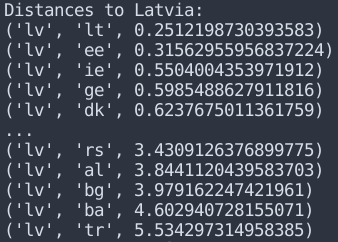
\includegraphics[height=4cm,page=1]{close-far-lv-classifier.png}
    \caption{Klasifikatora distances - Latvijai}
\end{figure}
\begin{figure}[h!]
    \centering
    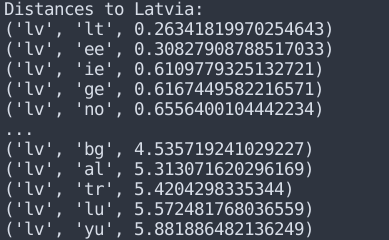
\includegraphics[height=4cm,page=1]{close-far-lv-model.png}
    \caption{Vidējo vērtību matricas distances - Latvijai}
\end{figure}

Droši vien pārsteidzošākais secinājums, ja var ticēt iegūtajiem rezultātiem, ir tas, ka pie gandrīz jebkuriem parametriem, viena no stiprākajām "kaimiņu būšanām" ir tieši Latvijai un Lietuvai. Protams, Balkāni veido cieši saistītu grafu, taču savstarpējā favorītisma ziņā laikam tomēr iepaliek. Tāpat saraksta augšgalā gandrīz vienmēr ir Rumānija ar Moldovu un Albānija ar (Ziemeļ)Maķedoniju.


\begin{figure}[h!]
    \centering
    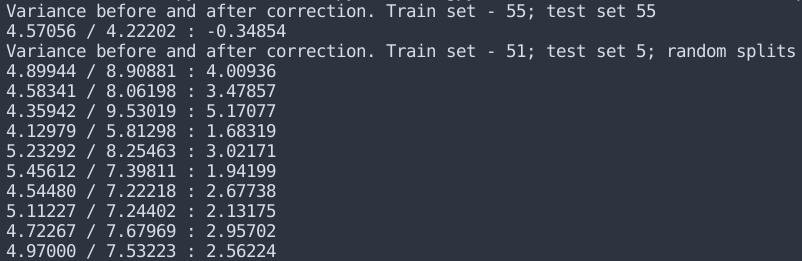
\includegraphics[height=5cm]{output-variance-bad.png}
    \caption{Dispersijas izmaiņas - reizinot ar $c_{ij}$}
\end{figure}
\newpage
\begin{figure}[h!]
    \centering
    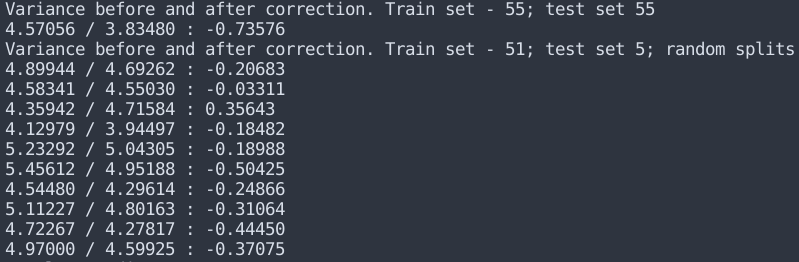
\includegraphics[height=5cm,page=1]{output-variance.png}
    \caption{Dispersijas izmaiņas - reizinot ar $\sqrt{c_{ij}}$}
\end{figure}

Salīdzinot datu kopu dispersijas (vidējās vērtība korpusam kopumā no 2-dimensionālo sadalījumu dispersijām katra etapa ietvaros), redzams, ka, vienkārši reizinot ar korekcijām, pārkārtojot pašu treniņa kopu un pārrēķinot rangus, dispersija samazinās, taču to pašu darot ar datiem, kas neietilpst treniņa sadalī-jumā, dispersija pieaug. Savukārt reizinot ar korekcijas kvadrātsakni, dispersija krītas abos gadījumos - arī datiem, kas treniņa kopā nav iekļauti. Pastāv divas visai ticamas iespējas:

\begin{itemize}
    \item Ir kāda vienkārša (vai ne tik vienkārša) matemātiska sakarība, kas determinēti nosaka, ka tā jābūt, bet patstāvīgā darba autors savos neveiklajos un kļūdpilnajos aprēķinos to vienkārši nav pamanījis. Tam varētu būt saistība ar divkāršo koeficientu rēķināšanu - vispirms vienādojot rindu varbūtību summas, tad līmeņojot tās lokāli;
    \item Notiek kaut kas analoģisks \textit{overfitting} - koriģējot ar pilnajām vērtībām tiek izdarīts par daudz, rezultāti tiek samudžināti un kropļoti. Tieši šī intuīcija ir tas, kas iedvesmoja veikt šādu (autoraprāt) matemātiski nepamatotu pārveidojumu, turklāt pat pirms dispersiju salīdzināšanas. Laimīgas sagadīšanās rezultātā šī korekcija patiešām izrādījās noderīga. Tas ir, ja šāds dispersiju izmaiņas novērtējums vispār kaut ko nozīmē - kas nebūt nav garantēts.
\end{itemize}

Izmēģināti trīs dažādi vizualizācijas paņēmieni - \textit{MDS}, \textit{isoMDS} un \textit{t-SNE}. Trešais nekādus saprotamus rezultātus sniegt nespēja, tāpēc netiek iekļauts. Pilna izmēra attēli atrodami projekta repozitorijā ``tex/'' direktorijā, kur ir arī šīs atskaites \LaTeX pirmokds.
\newpage
\begin{figure}[h!]
    \centering
    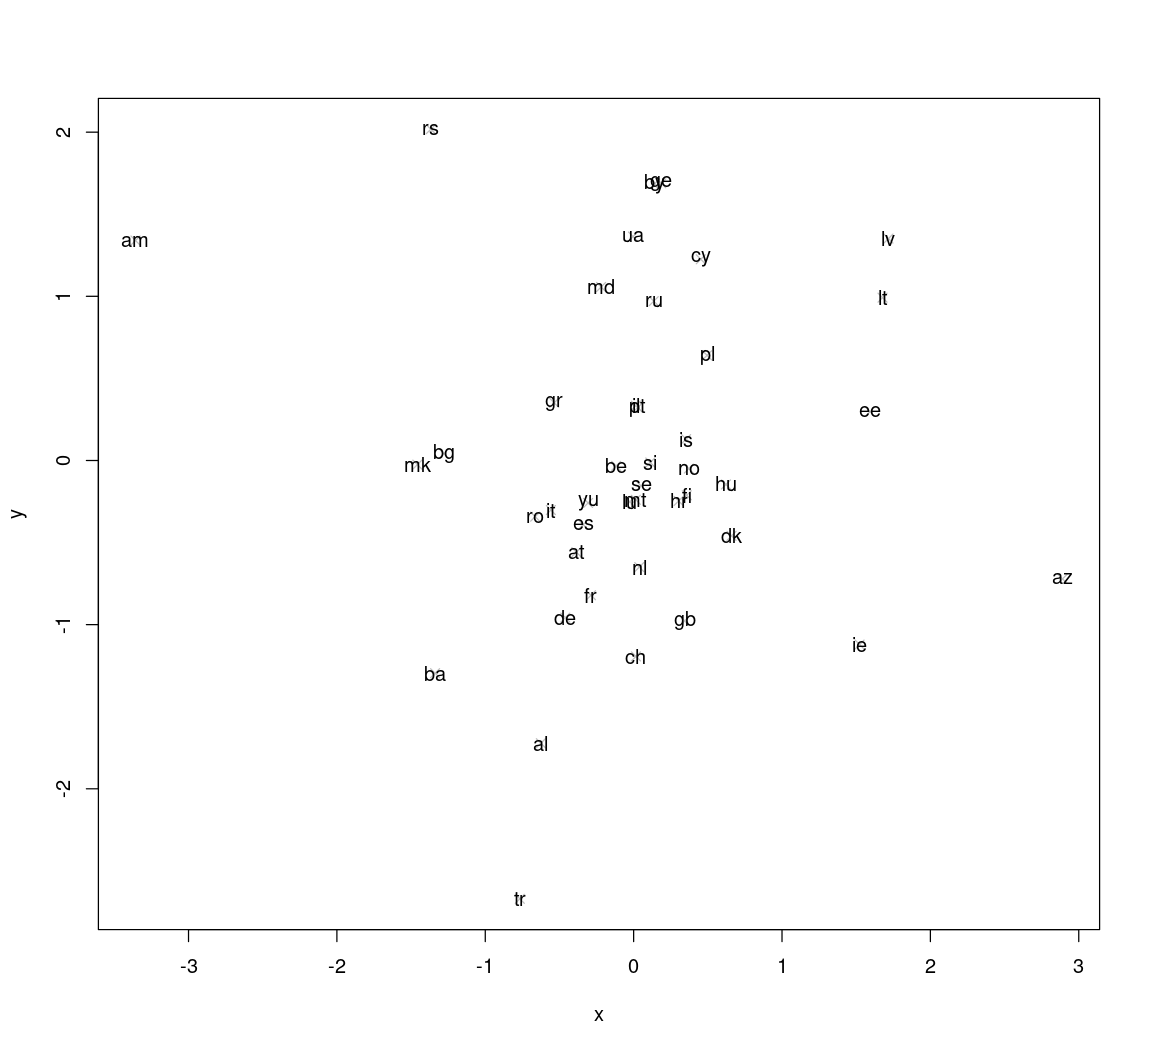
\includegraphics[height=11cm,page=1]{mds-classifier.png}
    \caption{MDS vizualizācija klasifikatora distancēm}
\end{figure}
\begin{figure}[h!]
    \centering
    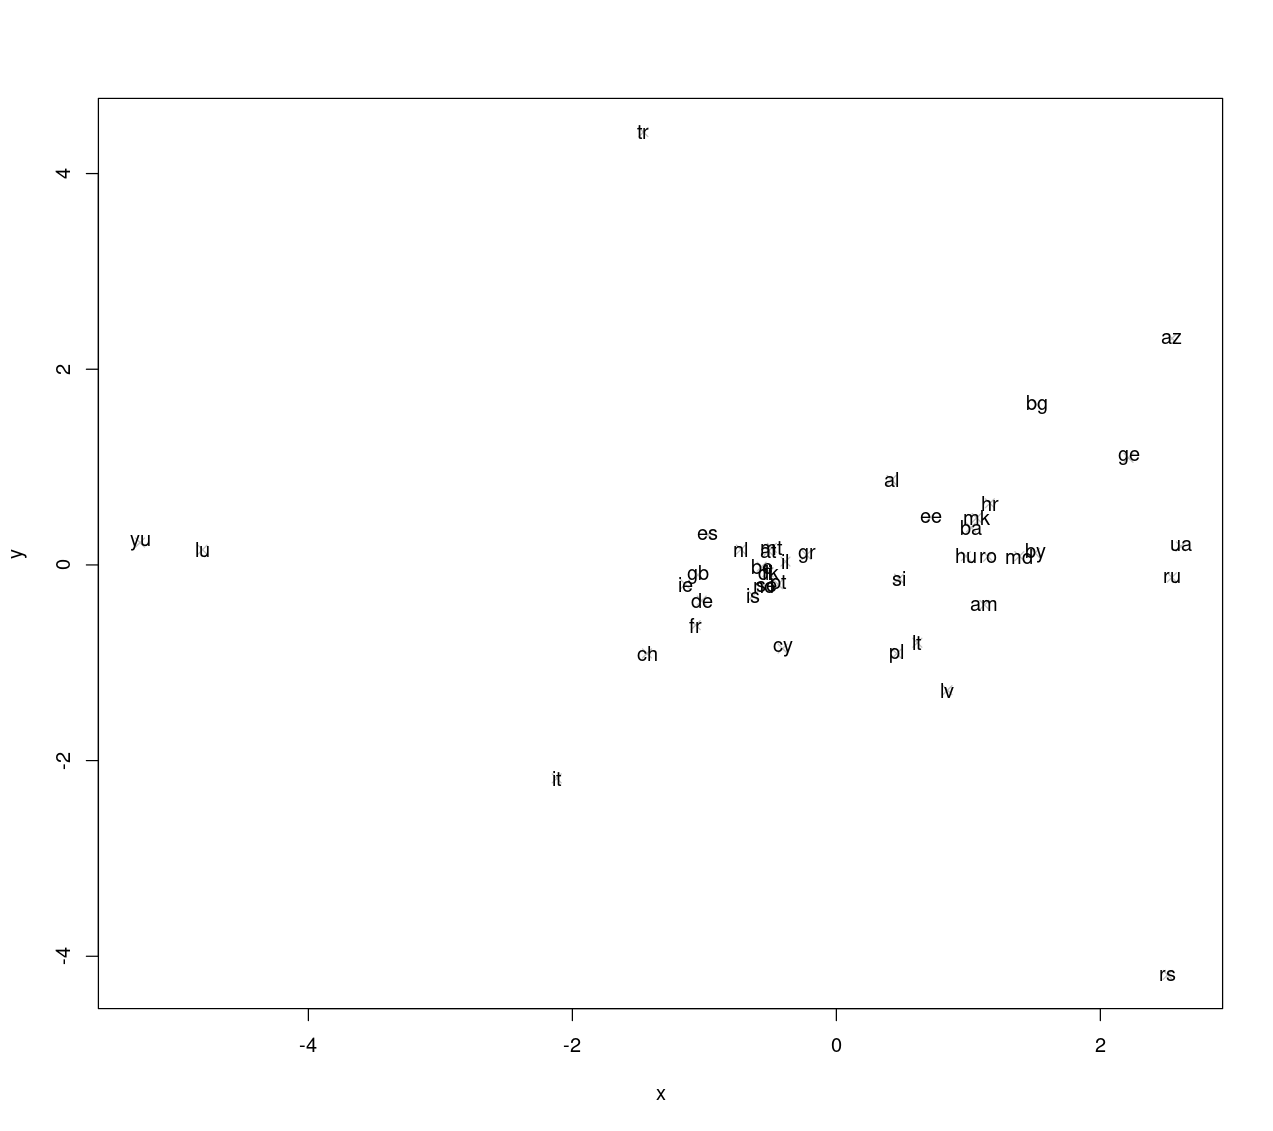
\includegraphics[height=11cm,page=1]{mds-model.png}
    \caption{MDS vizualizācija aprēķinu modeļa distancēm}
\end{figure}
\newpage

\begin{figure}[h!]
    \centering
    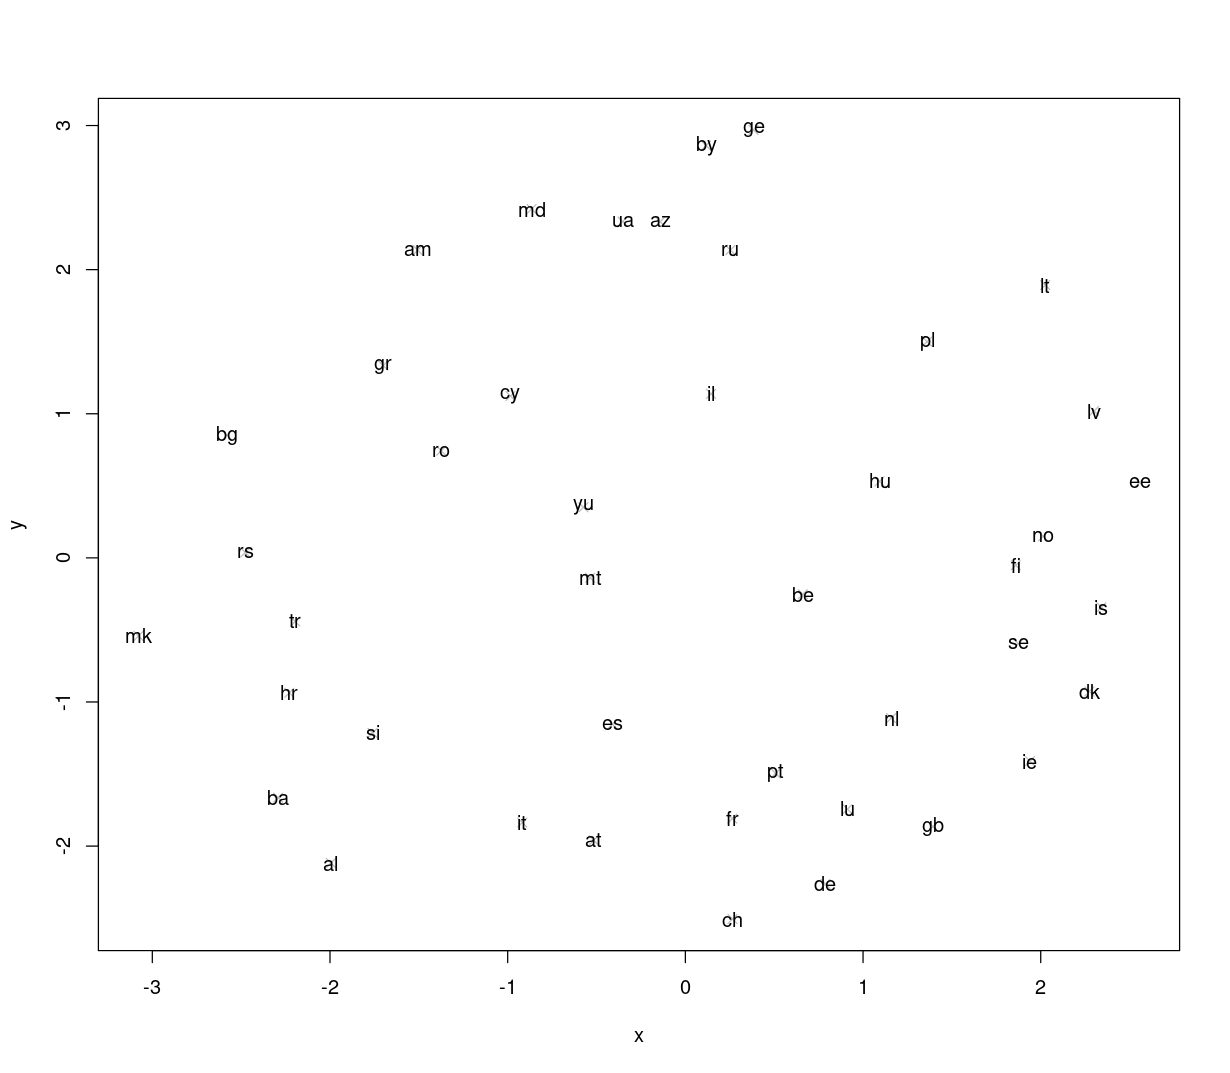
\includegraphics[height=11cm,page=1]{iso-mds-classifier.png}
    \caption{isoMDS vizualizācija klasifikatora distancēm}
\end{figure}
\begin{figure}[h!]
    \centering
    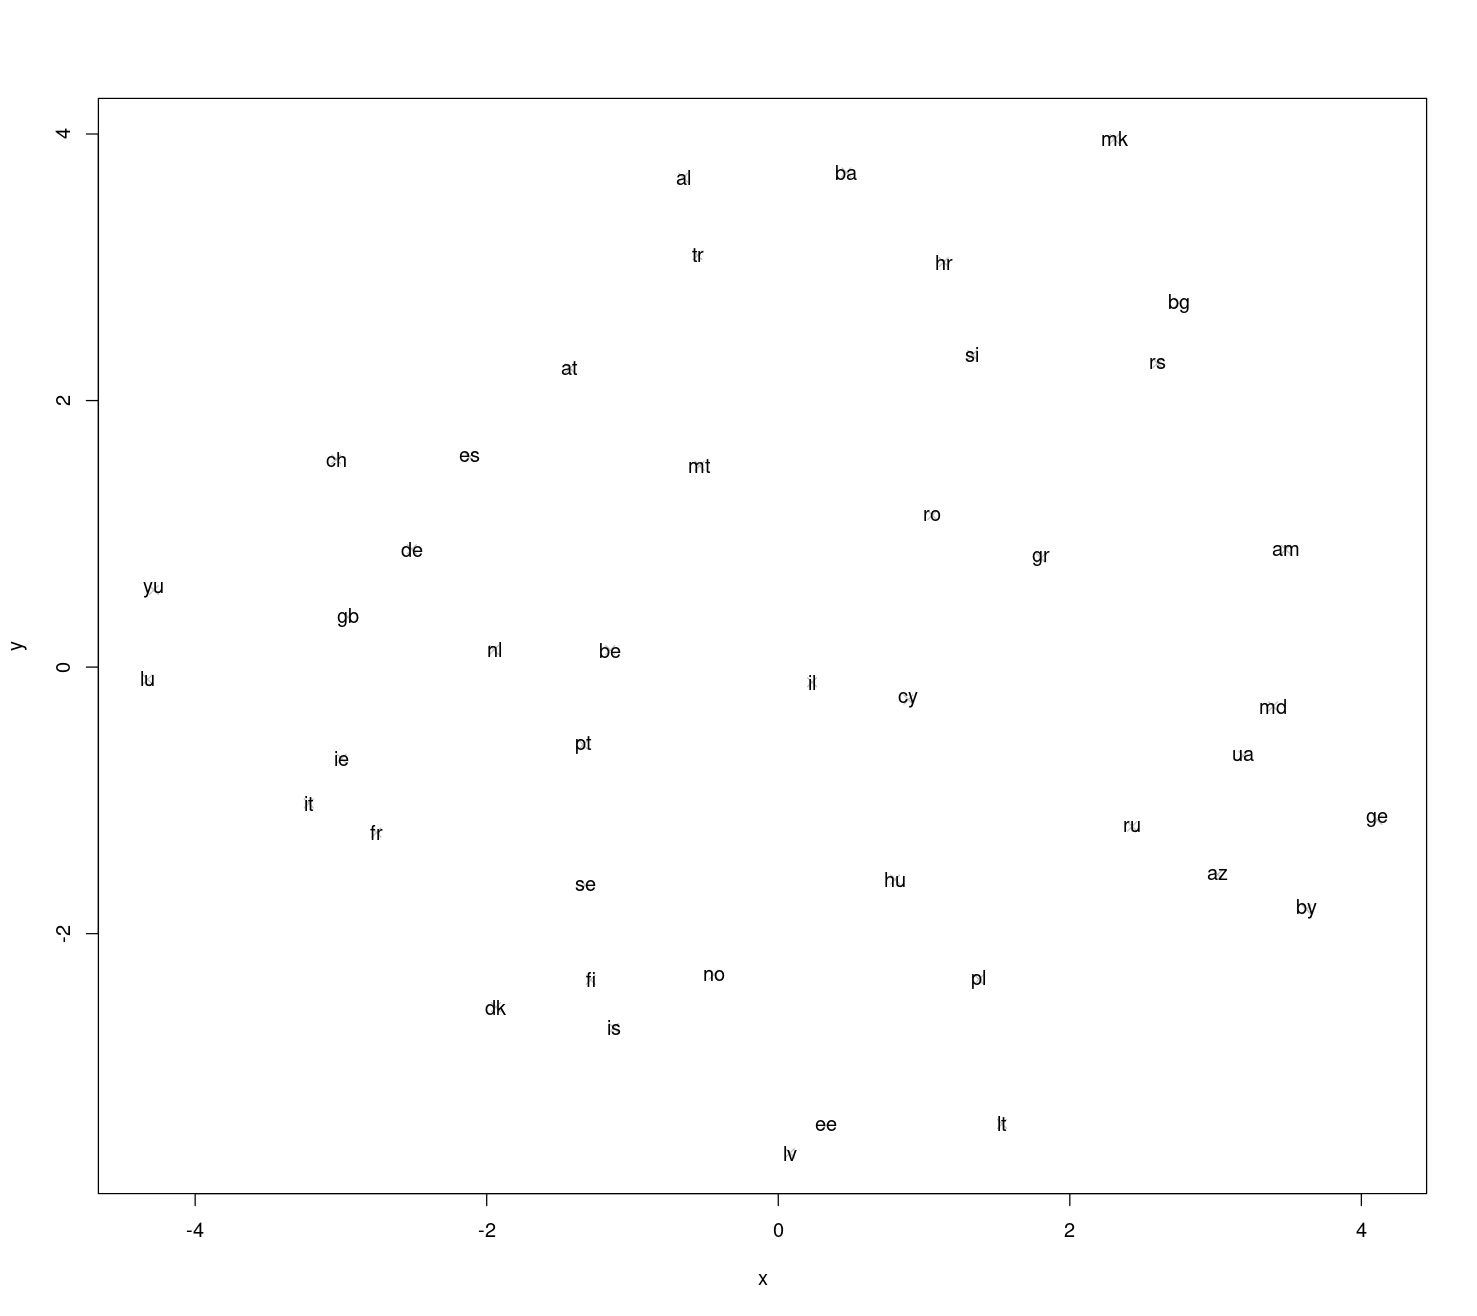
\includegraphics[height=11cm,page=1]{iso-mds-model.png}
    \caption{isoMDS vizualizācija aprēķinu modeļa distancēm}
\end{figure}
\newpage

Redzams, ka MDS gadījumā atrastā projekcija ir visnotaļ nevienmērīga, ar klasteriem tuvu koordinātu sākumpunktam un izlēcējiem. \textit{isoMDS} iegūst daudz vienmērīgāku izkliedi. Abos gadījumos tomēr ir redzams, kā, piemēram, Balkānu, Skandināvijas, Austrumeiropas (tās šaurajā definīcijā) vai Baltijas valstis grupējas.

\section{Secinājumi}

Darba gaitā tika diezgan detalizēti iepazīta konkrēta datu kopa - Eirovīzijas dziesmu konkursa rezultāti (precīzāk, laika periodā starp 1980. un 2015. gadu, kad vērtēšana notika pēc vienāda principa vai vismaz pietiekami nemainīga principa), izvirzīta hipotēze par ģenerējošo modeli t.s. ``kaimiņu būšanas" fenomenam, piedāvāta metode tā koriģē-šanai. Praktiski tika izstrādāti skripti gan tipveida klasifikatora ģeneratora pielietojumam, gan datu kopas elementārai algebriskai reducēšanai uz formu, kurā aprēķins būtu izsakāms analītiski.

Rezultātā tika iegūti ``kaimiņu būšanas'' novērtējumi no diviem radikāli atšķirīgiem modeļiem, kas tomēr daudzējādā ziņā ir līdzīgi. To ģenerēto skaitlisko vērtību un vizualizā-ciju pārbaude atklāj likumsakarības, kas sakrīt ar cilvēka intuitīvo izpratni par meklējamās parādības būtību. Piedāvātajai korekcijas metodei tika arī izstrādāts kvantitatīvs novērtē-jums, taču par tā nozīmīgumu ir grūti spriest, jo, tāpat kā pati aprēķinu secība, kas noved pie modeļa, tas nav nekā dziļi matemātiski pamatots.

\end{document}